\documentclass{standalone}
\usepackage{tikz}
\usetikzlibrary{patterns, positioning}


\begin{document}
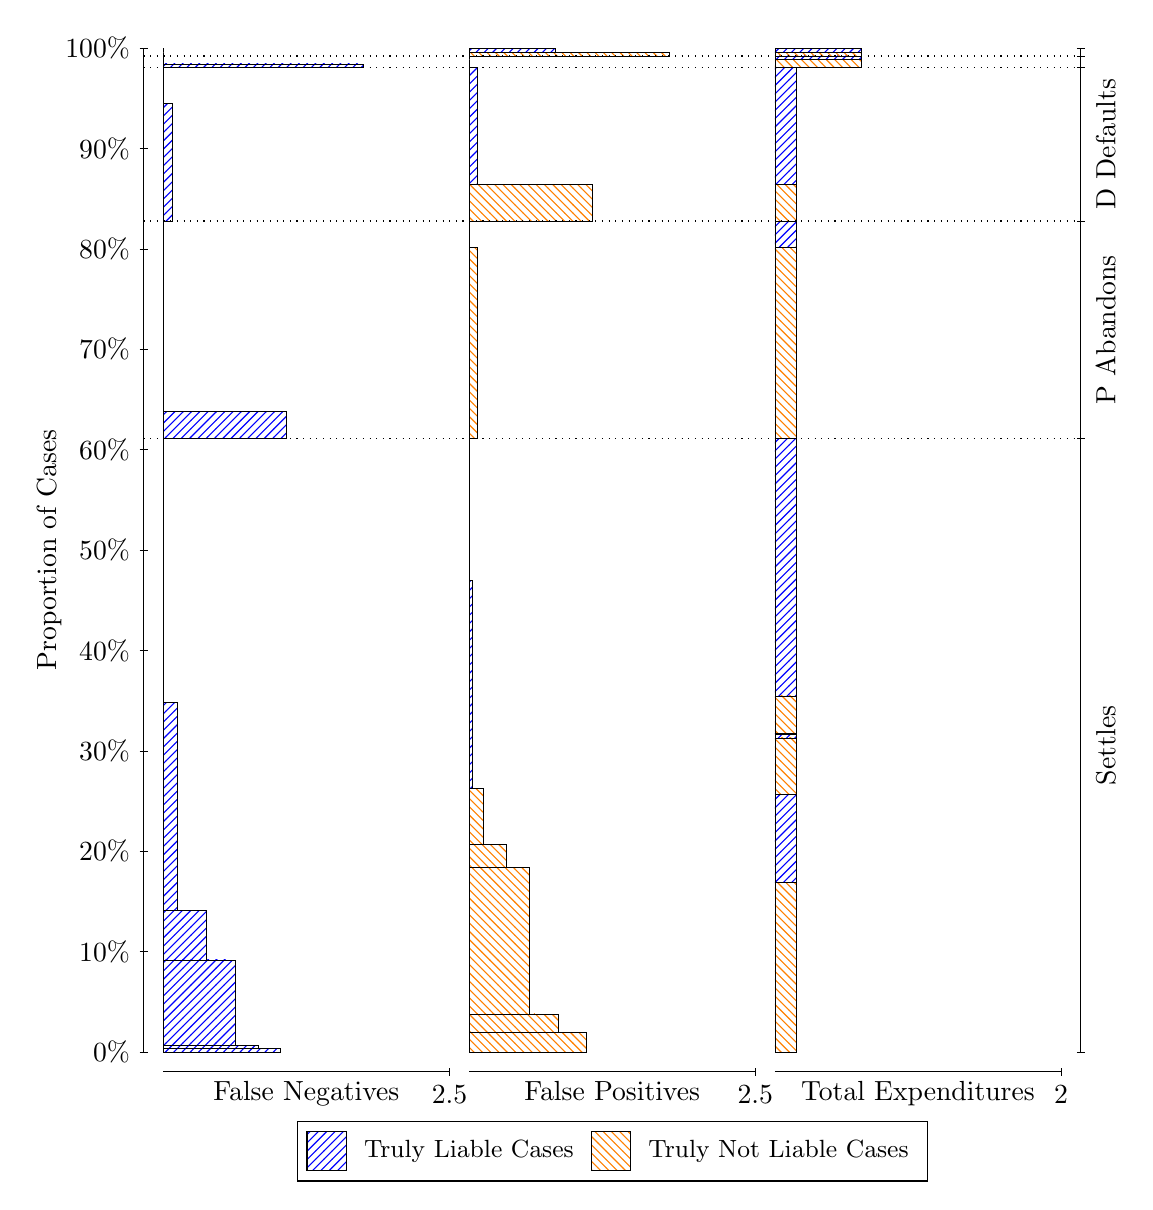
\begin{tikzpicture}
\draw[black, very thin] (1.5,1.75) -- (1.5,14.5);
\node[rotate=90, text=black, anchor=center] at (0.3, 8.125) {Proportion of Cases};
\draw[black, very thin] (1.45,1.75) -- (1.55,1.75);
\node[text=black, anchor=east] at (1.45, 1.75) {0\%};
\draw[black, very thin] (1.45,3.025) -- (1.55,3.025);
\node[text=black, anchor=east] at (1.45, 3.025) {10\%};
\draw[black, very thin] (1.45,4.3) -- (1.55,4.3);
\node[text=black, anchor=east] at (1.45, 4.3) {20\%};
\draw[black, very thin] (1.45,5.575) -- (1.55,5.575);
\node[text=black, anchor=east] at (1.45, 5.575) {30\%};
\draw[black, very thin] (1.45,6.85) -- (1.55,6.85);
\node[text=black, anchor=east] at (1.45, 6.85) {40\%};
\draw[black, very thin] (1.45,8.125) -- (1.55,8.125);
\node[text=black, anchor=east] at (1.45, 8.125) {50\%};
\draw[black, very thin] (1.45,9.4) -- (1.55,9.4);
\node[text=black, anchor=east] at (1.45, 9.4) {60\%};
\draw[black, very thin] (1.45,10.675) -- (1.55,10.675);
\node[text=black, anchor=east] at (1.45, 10.675) {70\%};
\draw[black, very thin] (1.45,11.95) -- (1.55,11.95);
\node[text=black, anchor=east] at (1.45, 11.95) {80\%};
\draw[black, very thin] (1.45,13.225) -- (1.55,13.225);
\node[text=black, anchor=east] at (1.45, 13.225) {90\%};
\draw[black, very thin] (1.45,14.5) -- (1.55,14.5);
\node[text=black, anchor=east] at (1.45, 14.5) {100\%};

\draw[black, very thin] (13.4,1.75) -- (13.4,14.5);
\draw[black, very thin] (13.35,1.75) -- (13.45,1.75);
\node[anchor=west] at (13.35, 1.75) {};
\draw[black, very thin] (13.35,9.5435) -- (13.45,9.5435);
\node[anchor=west] at (13.35, 9.5435) {};
\draw[black, very thin] (13.35,12.303) -- (13.45,12.303);
\node[anchor=west] at (13.35, 12.303) {};
\draw[black, very thin] (13.35,14.256) -- (13.45,14.256);
\node[anchor=west] at (13.35, 14.256) {};
\draw[black, very thin] (13.35,14.399) -- (13.45,14.399);
\node[anchor=west] at (13.35, 14.399) {};
\draw[black, very thin] (13.35,14.5) -- (13.45,14.5);
\node[anchor=west] at (13.35, 14.5) {};

\draw[black, very thin, pattern color=blue, pattern=north east lines] (1.75,1.75) rectangle (3.2397,1.7938);
\draw[black, very thin, pattern color=blue, pattern=north east lines] (1.75,1.7938) rectangle (2.949,1.8341);
\draw[black, very thin, pattern color=blue, pattern=north east lines] (1.75,1.8341) rectangle (2.6583,2.9156);
\draw[black, very thin, pattern color=blue, pattern=north east lines] (1.75,2.9156) rectangle (2.5857,2.9205);
\draw[black, very thin, pattern color=blue, pattern=north east lines] (1.75,2.9205) rectangle (2.295,3.5506);
\draw[black, very thin, pattern color=blue, pattern=north east lines] (1.75,3.5506) rectangle (1.9317,6.1928);
\draw[black, very thin, pattern color=orange, pattern=north west lines] (1.75,6.1928) rectangle (1.75,9.5435);
\draw[black, very thin, pattern color=blue, pattern=north east lines] (1.75,9.5435) rectangle (3.3123,9.8828);
\draw[black, very thin, pattern color=orange, pattern=north west lines] (1.75,9.8828) rectangle (1.75,12.303);
\draw[black, very thin, pattern color=blue, pattern=north east lines] (1.75,12.303) rectangle (1.859,13.795);
\draw[black, very thin, pattern color=orange, pattern=north west lines] (1.75,13.795) rectangle (1.75,14.256);
\draw[black, very thin, pattern color=blue, pattern=north east lines] (1.75,14.256) rectangle (4.2933,14.299);
\draw[black, very thin, pattern color=orange, pattern=north west lines] (1.75,14.299) rectangle (1.75,14.399);
\draw[black, very thin, pattern color=orange, pattern=north west lines] (1.75,14.399) rectangle (1.75,14.441);
\draw[black, very thin, pattern color=blue, pattern=north east lines] (1.75,14.441) rectangle (1.75,14.5);
\draw[black, very thin, pattern color=orange, pattern=north west lines] (5.6333,1.75) rectangle (7.123,2.0016);
\draw[black, very thin, pattern color=orange, pattern=north west lines] (5.6333,2.0016) rectangle (6.7597,2.2252);
\draw[black, very thin, pattern color=orange, pattern=north west lines] (5.6333,2.2252) rectangle (6.469,2.2345);
\draw[black, very thin, pattern color=orange, pattern=north west lines] (5.6333,2.2345) rectangle (6.3963,4.0991);
\draw[black, very thin, pattern color=orange, pattern=north west lines] (5.6333,4.0991) rectangle (6.1057,4.3863);
\draw[black, very thin, pattern color=orange, pattern=north west lines] (5.6333,4.3863) rectangle (5.815,5.1007);
\draw[black, very thin, pattern color=blue, pattern=north east lines] (5.6333,5.1007) rectangle (5.6697,7.7429);
\draw[black, very thin, pattern color=blue, pattern=north east lines] (5.6333,7.7429) rectangle (5.6333,9.5435);
\draw[black, very thin, pattern color=orange, pattern=north west lines] (5.6333,9.5435) rectangle (5.7423,11.964);
\draw[black, very thin, pattern color=blue, pattern=north east lines] (5.6333,11.964) rectangle (5.6333,12.303);
\draw[black, very thin, pattern color=orange, pattern=north west lines] (5.6333,12.303) rectangle (7.1957,12.765);
\draw[black, very thin, pattern color=blue, pattern=north east lines] (5.6333,12.765) rectangle (5.7423,14.256);
\draw[black, very thin, pattern color=orange, pattern=north west lines] (5.6333,14.256) rectangle (5.6333,14.356);
\draw[black, very thin, pattern color=blue, pattern=north east lines] (5.6333,14.356) rectangle (5.6333,14.399);
\draw[black, very thin, pattern color=orange, pattern=north west lines] (5.6333,14.399) rectangle (8.1767,14.441);
\draw[black, very thin, pattern color=blue, pattern=north east lines] (5.6333,14.441) rectangle (6.7233,14.5);
\draw[black, very thin, pattern color=orange, pattern=north west lines] (9.5167,1.75) rectangle (9.7892,3.9018);
\draw[black, very thin, pattern color=blue, pattern=north east lines] (9.5167,3.9018) rectangle (9.7892,5.0236);
\draw[black, very thin, pattern color=orange, pattern=north west lines] (9.5167,5.0236) rectangle (9.7892,5.738);
\draw[black, very thin, pattern color=blue, pattern=north east lines] (9.5167,5.738) rectangle (9.7892,5.7818);
\draw[black, very thin, pattern color=orange, pattern=north west lines] (9.5167,5.7818) rectangle (9.7892,5.791);
\draw[black, very thin, pattern color=blue, pattern=north east lines] (9.5167,5.791) rectangle (9.7892,5.796);
\draw[black, very thin, pattern color=orange, pattern=north west lines] (9.5167,5.796) rectangle (9.7892,6.2712);
\draw[black, very thin, pattern color=blue, pattern=north east lines] (9.5167,6.2712) rectangle (9.7892,9.5435);
\draw[black, very thin, pattern color=orange, pattern=north west lines] (9.5167,9.5435) rectangle (9.7892,11.964);
\draw[black, very thin, pattern color=blue, pattern=north east lines] (9.5167,11.964) rectangle (9.7892,12.303);
\draw[black, very thin, pattern color=orange, pattern=north west lines] (9.5167,12.303) rectangle (9.7892,12.765);
\draw[black, very thin, pattern color=blue, pattern=north east lines] (9.5167,12.765) rectangle (9.7892,14.256);
\draw[black, very thin, pattern color=orange, pattern=north west lines] (9.5167,14.256) rectangle (10.607,14.356);
\draw[black, very thin, pattern color=blue, pattern=north east lines] (9.5167,14.356) rectangle (10.607,14.399);
\draw[black, very thin, pattern color=orange, pattern=north west lines] (9.5167,14.399) rectangle (10.607,14.441);
\draw[black, very thin, pattern color=blue, pattern=north east lines] (9.5167,14.441) rectangle (10.607,14.5);
\draw[black, dotted] (1.5,9.5435) -- (13.4,9.5435);
\draw[black, dotted] (1.5,12.303) -- (13.4,12.303);
\draw[black, dotted] (1.5,14.256) -- (13.4,14.256);
\draw[black, dotted] (1.5,14.399) -- (13.4,14.399);
\draw[black, very thin] (1.75,1.5) -- (5.3833,1.5);
\node[text=black, anchor=north] at (3.5667, 1.5) {False Negatives};
\draw[black, very thin] (5.3833,1.45) -- (5.3833,1.55);
\node[text=black, anchor=north] at (5.3833, 1.45) {2.5};

\draw[black, very thin] (5.6333,1.5) -- (9.2667,1.5);
\node[text=black, anchor=north] at (7.45, 1.5) {False Positives};
\draw[black, very thin] (9.2667,1.45) -- (9.2667,1.55);
\node[text=black, anchor=north] at (9.2667, 1.45) {2.5};

\draw[black, very thin] (9.5167,1.5) -- (13.15,1.5);
\node[text=black, anchor=north] at (11.333, 1.5) {Total Expenditures};
\draw[black, very thin] (13.15,1.45) -- (13.15,1.55);
\node[text=black, anchor=north] at (13.15, 1.45) {2};

\node[text=black, centered, rotate=90] at (13.72, 5.6467) {Settles};
\node[text=black, centered, rotate=90] at (13.72, 10.923) {P Abandons};
\node[text=black, centered, rotate=90] at (13.72, 13.28) {D Defaults};



\draw (7.449999999999999,1.5) node[draw=none] (baseCoordinate) {};
\begin{scope}[align=center]
        \matrix[scale=0.5, draw=black, below=0.5cm of baseCoordinate, nodes={draw}, column sep=0.1cm]{
            \node[rectangle, draw, minimum width=0.5cm, minimum height=0.5cm, pattern color=blue, pattern=north east lines] {}; &
            \node[draw=none, font=\small, text=black] (B) {Truly Liable Cases}; &
            \node[rectangle, draw, minimum width=0.5cm, minimum height=0.5cm, pattern color=orange, pattern=north west lines] {}; &
            \node[draw=none, font=\small, text=black] (B) {Truly Not Liable Cases}; \\
            };
\end{scope}

\end{tikzpicture}
\end{document}